\section{Results} \label{sec:results}

The mass of the weights were calculated using digital weights: $M = 29.9 \pm 0.1 (g)$.
\begin{equation*}
  \left\langle M \right\rangle = \frac{1}{N}\sum\limits_{i=1}^{N}M_{i} = 29.9 (g)
\end{equation*}
\begin{equation*}
  \Delta M = \frac{1}{N}\sqrt{\sum\limits_{i=1}^{N}(M_{i} - \left\langle M \right\rangle)^{2}} = 0.1 (g)
\end{equation*}

As discussed in section \ref{sec:discussion}, weights were attached to either ends of the gyroscope. However, weight's position was pushed towards the gyroscope vertical axis due to rotations (see \ref{fig:results:locs}). Three possible locations were measured using vernier callipers to be:
\begin{equation*}
  \left\langle l_{I} \right\rangle = \frac{1}{N}\sum\limits_{i=1}^{N}l_{Ii} = 33.0 (cm)
\end{equation*}
\begin{equation*}
  \Delta l_{I} = \frac{1}{N}\sqrt{\sum\limits_{i=1}^{N}(l_{Ii} - \left\langle l_{I} \right\rangle)^{2}} = 0.4 (cm)
\end{equation*}

Thus, $l_{I} = 33.0 \pm 0.4 (cm)$. Similarly, $l_{II} = 19.7 \pm 0.1 (cm)$ and $l_{III} = 23.9 \pm 0.1 (cm)$.

\emph{TISensorTag} was recording precession frequency ($\boldsymbol\Omega$) of the gyroscope (vertical axis) for different torques\footnote{Torque is specified by the mass of the weight and the lever arm length where the weight was attached with respect to the vertical axis of the gyroscope.} and different spinning angular velocities $\boldsymbol\omega_{3}$. This data is shown in table \ref{tab:results:precession} for each point (see appendix \ref{sec:appendix:precession_raw_data} for more details about precession frequency data, and appendix \ref{appendix:errors} for detailed error analysis).

\begin{table}[ht!]
  \centering
  \begin{tabular}{|c|c|c|c|c|}
    Point & Type & Precession ($\boldsymbol\Omega$), $\frac{rad}{s}$ & Mass ($M$), $g$ & Lever Arm Length ($l$), $cm$ \\ \hline
    $\#1$ & $II$ & $0.449711 \pm 0.031443$ & $59.8 \pm 0.2$ & $19.7 \pm 0.1$ \\ \hline
    $\#2$ & $II$ & $0.716604 \pm 0.055174$ & $59.8 \pm 0.2$ & $33.0 \pm 0.4$ \\ \hline
    $\#3$ & $II$ & $0.18821 \pm 0.02623$   & $29.9 \pm 0.1$ & $23.9 \pm 0.1$ \\ \hline
    $\#4$ & $II$ & $0.56268 \pm 0.06639$   & $59.8 \pm 0.2$ & $33.0 \pm 0.4$ \\ \hline
    $\#5$ & $I$  & $0.528033 \pm 0.005273$ & $29.9 \pm 0.1$ & $33.2 \pm 0.4$ \\ \hline
    $\#6$ & $I$  & $0.258233 \pm 0.002976$ & $29.9 \pm 0.1$ & $33.2 \pm 0.4$ \\ \hline
    $\#7$ & $I$  & $0.165118 \pm 0.000843$ & $59.8 \pm 0.2$ & $19.7 \pm 0.1$ \\ \hline
  \end{tabular}
  \caption{Precession frequencies ($\Omega$)}
  \label{tab:results:precession}
\end{table}


In the first part of the experiment the rotor’s behavior without external forces was observed, for this the rotor was rotated by hand. After this the base was rotated, during the rotation of the base the rotor remained stationary. This is caused by conservation of angular momentum. Angular momentum conservation also explains why it is only possible to throw a flat object over a long distance if it has spin; a spinning object resists changes in its orientation, this stabilizes the object's flight and keeps it flat, reducing wobbling.
The gyroscope would only precess if a torque was applied to it, this was done by adding weights to the setup. The weight had a mass of $(29.9 \pm 0.1)*10^-3 kg,$ the masses were placed at distances of $19.9 \pm 0.1 cm$ and $33.2 \pm 0.4 cm$ from the vertical axis of the gyroscope.
Next the moment of inertia of the rotor around its own axis was determined, this was done using the equation:
\begin{equation*}
    I_3 = \frac{1}{2} M_d R_d^2
\end{equation*}
Where $M_d$ is the mass of the rotor disc, this was given to be $1.74 kg$ and $R_d$ is the radius of the disc, which was $12.47 \pm 0.04 cm$. Substituting in the values of $M_d$ and $R_d$ gave $I_3 = 0.0271 \pm 0.0004 kgm^2$. After this $T_3$ was calculated by the following equation:
\begin{equation*}
    T_3 = \frac{10}{Ar}
\end{equation*}
Where $Ar$ is the average rotaions per 10 seconds, which was determined by filming the setup an dividing the film in 10 second long clips, counting the rotations per clip and then taking the average. The differnt values of $T_3$ are shown in Table x in the appendix. The previous measured components were used to calculate $T_{p, \text{calculated}}$ using:
\begin{equation*}
    T_{p, \text{calculated}} = \frac{4\pi^2I_3}{MglT_3}
\end{equation*}
$T_{p, \text{measured}}$ was calculated using:
\begin{equation*}
    T_{p, \text{measured}} = \frac{2\pi}{\Omega}
\end{equation*}
$T_{p, \text{calculated}}$ was plotted against $T_{p, \text{measured}}$ in \ref{fig:gyro}.

\begin{figure}[h!]
    \centering
    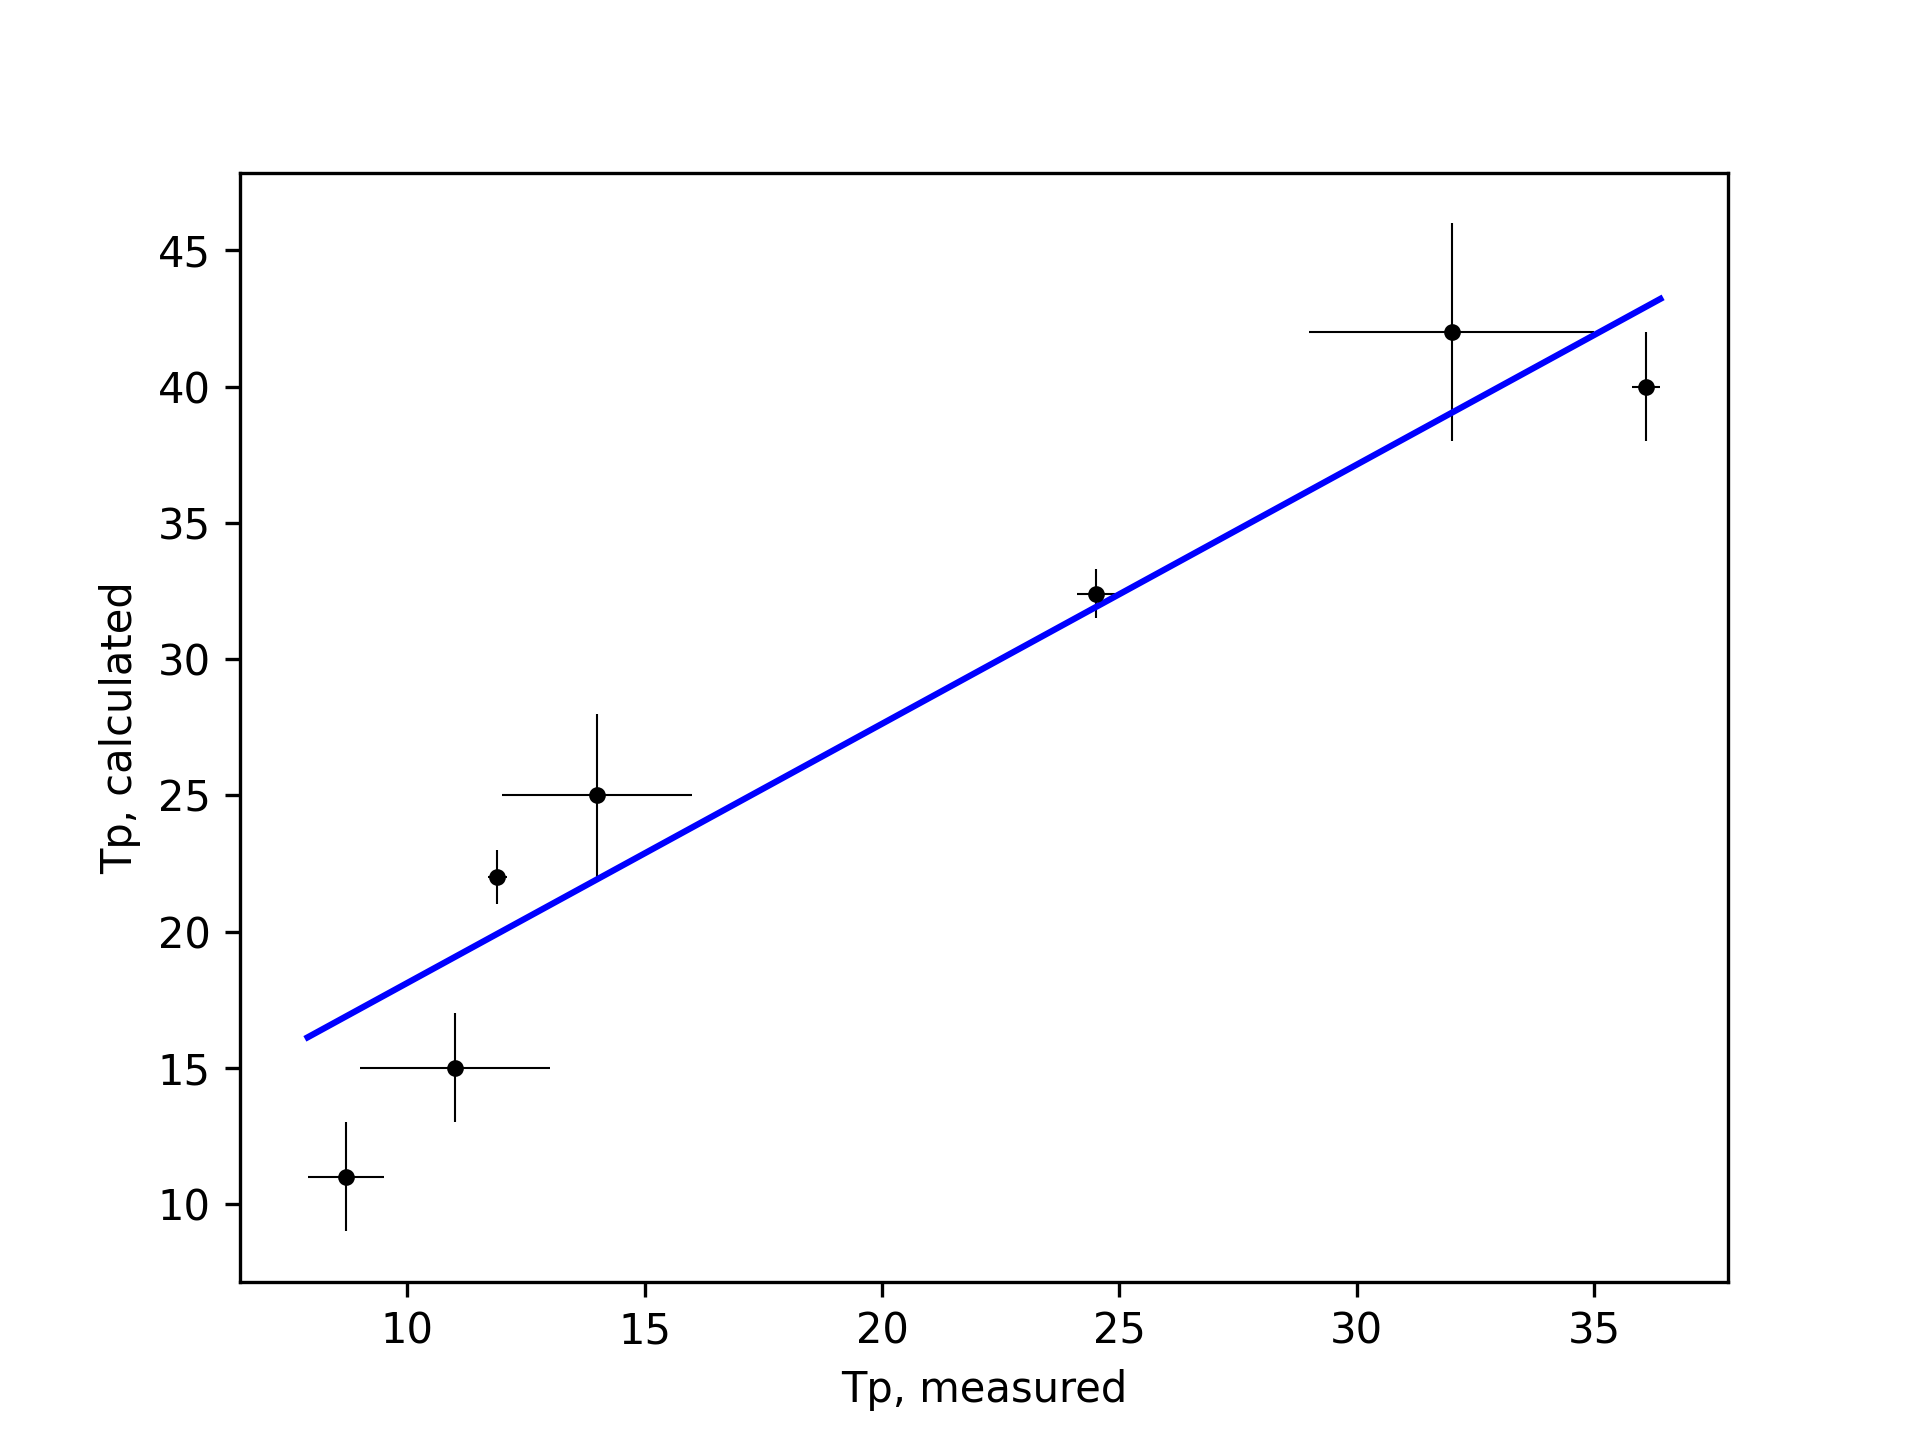
\includegraphics[width=0.8\textwidth]{gyroscope/images/gyro}
    \caption{Correlation between calculated and measured precession periods}
    \label{fig:gyro}
\end{figure}

The line of best fit has a slope of $1.0 \pm 0.2$.
